\section{Example from the literature}
\label{sec:example}

We use the following example to demonstrate how we find the homeostasis 
conditions using mainly the network topology. The example used is original 
from \cite{wang2021} and showed in Fig.\ref{fig:fig1}.

\begin{figure}[H]
    \centering
    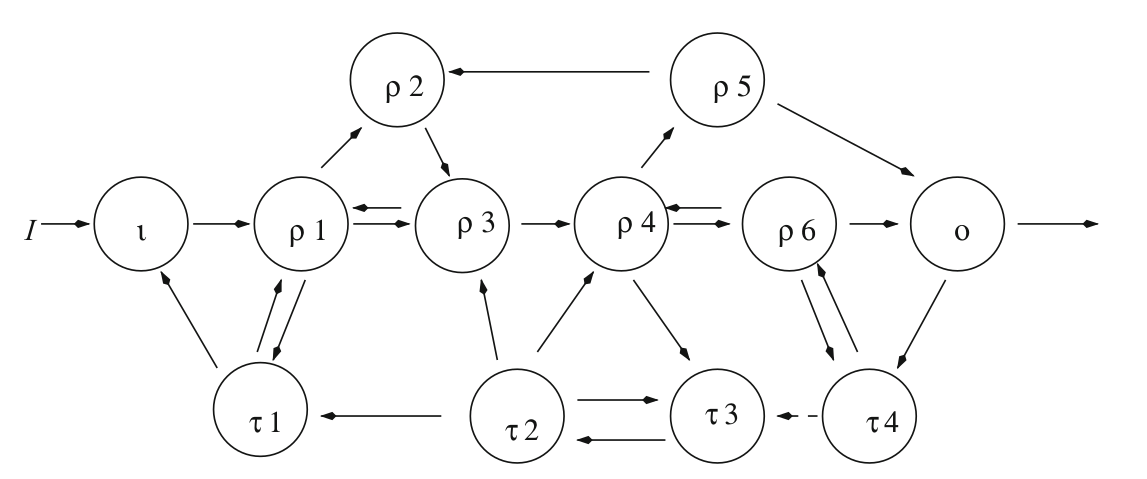
\includegraphics[scale=0.36]{figs/fig2_example.png}
    \caption{12-node example. Source: \cite{wang2021}}
    \label{fig:fig1}
\end{figure}

Using the notation provided by \cite{wang2021} we have that the
\textbf{simple nodes} are $(\rho_1, \rho_2, \rho_3, \rho_4, \rho_5, \rho_6)$,
the \textbf{appendage nodes} are $(\tau_1, \tau_2, \tau_3, \tau_4)$ and the 
\textbf{super-simple nodes} are $\mathcal{I}, \rho_1, \rho_3, \rho_4, \mathcal{O}$.
The \textbf{IO-simple paths} are 
\begin{equation}
    \begin{aligned}
        \mathcal{I}& \rightarrow \rho_1 \rightarrow \rho_2 
        \rightarrow \rho_3 \rightarrow \rho_4 \rightarrow \rho_5 \rightarrow \mathcal{O}\\
        \mathcal{I}& \rightarrow \rho_1 \rightarrow \rho_2 
        \rightarrow \rho_3 \rightarrow \rho_4 \rightarrow \rho_6 \rightarrow \mathcal{O}\\
        \mathcal{I}& \rightarrow \rho_1 
        \rightarrow \rho_3 \rightarrow \rho_4 \rightarrow \rho_5 \rightarrow \mathcal{O}\\
        \mathcal{I}& \rightarrow \rho_1 
        \rightarrow \rho_3 \rightarrow \rho_4 \rightarrow \rho_6 \rightarrow \mathcal{O}
    \end{aligned}
\end{equation}  

The classification above allows us to obtain the subnetworks showed in Fig.~\ref{fig:fig2}.
The subnetworks obtained are either appendage subnetworks or super-simple structural subnetworks
(more details is provided in \cite{wang2021}, but I can add more here if necessary).
Since each subnetwork obtained is associated with the blocks $B_j$ of the homeostasis
matrix $H$, we have that
\begin{equation}
    det(H) = det(B_1)det(B_2)det(B_3)
    det(B_4)det(B_5)det(B_6)
\end{equation}
where $B_1$ and $B_2$ are the Jacobian of the appendage subnetworks $A_1$ and $A_2$
and $B_3, B_4, B_5$ and $B_6$ are the homeostasis matrices of the super-simple 
structural subnetworks $H(\mathcal{L}(\mathcal{I}, \rho_1)$, 
$H(\mathcal{L}(\rho_1, \rho_3))$, $H(\mathcal{L}(\rho_3, \rho_4))$ and 
$H(\mathcal{L}(\rho_4, \mathcal{O}))$, respectively. Therefore, we have 
\begin{equation}
    J_{A_2} = 
    \begin{pmatrix}
        f_{\rho_2, \rho_2} & f_{\rho_2, \rho_3} \\
        f_{\rho_3, \rho_2} & f_{\rho_3, \rho_3}
    \end{pmatrix},
\end{equation}

\begin{equation}
    H(\mathcal{L}(\rho_1, \rho_3)) = 
    \begin{pmatrix}
        f_{\rho_2, \rho_1} & f_{\rho_2, \rho_2} \\
        f_{\rho_3, \rho_1} & f_{\rho_3, \rho_2}
    \end{pmatrix}
\end{equation}

\begin{equation}
    H(\mathcal{L}(\rho_4, \mathcal{O})) = 
    \begin{pmatrix}
        f_{\rho_5, \rho_4} & f_{\rho_5, \rho_5} & 0 & 0 \\
        f_{\rho_3, \rho_1} & 0 & f_{\rho_3, \rho_2} & f_{\rho_6,\rho_4}\\
        0 & 0 & f_{\rho_4, \rho_6} & f_{\rho_4, \rho_4}\\
        0 & f_{\mathcal{O}, \rho_5} & f_{\mathcal{O}, \rho_6} & 0\\
    \end{pmatrix}
\end{equation}
and $det(J_{A_1}) = f_{\tau_1, \tau_1}$, 
$det(H(\mathcal{L}(\mathcal{I}, \rho_1))) = f_{\rho_1, \mathcal{I}}$, 
and $det(H(\mathcal{L}(\rho_3, \rho_4))) = f_{\rho_4, \rho_3}$. Then, 
each condition $det(B_j) = 0$ determines an infinitesimal homeostasis
type.

\begin{figure}[H]
    \centering
    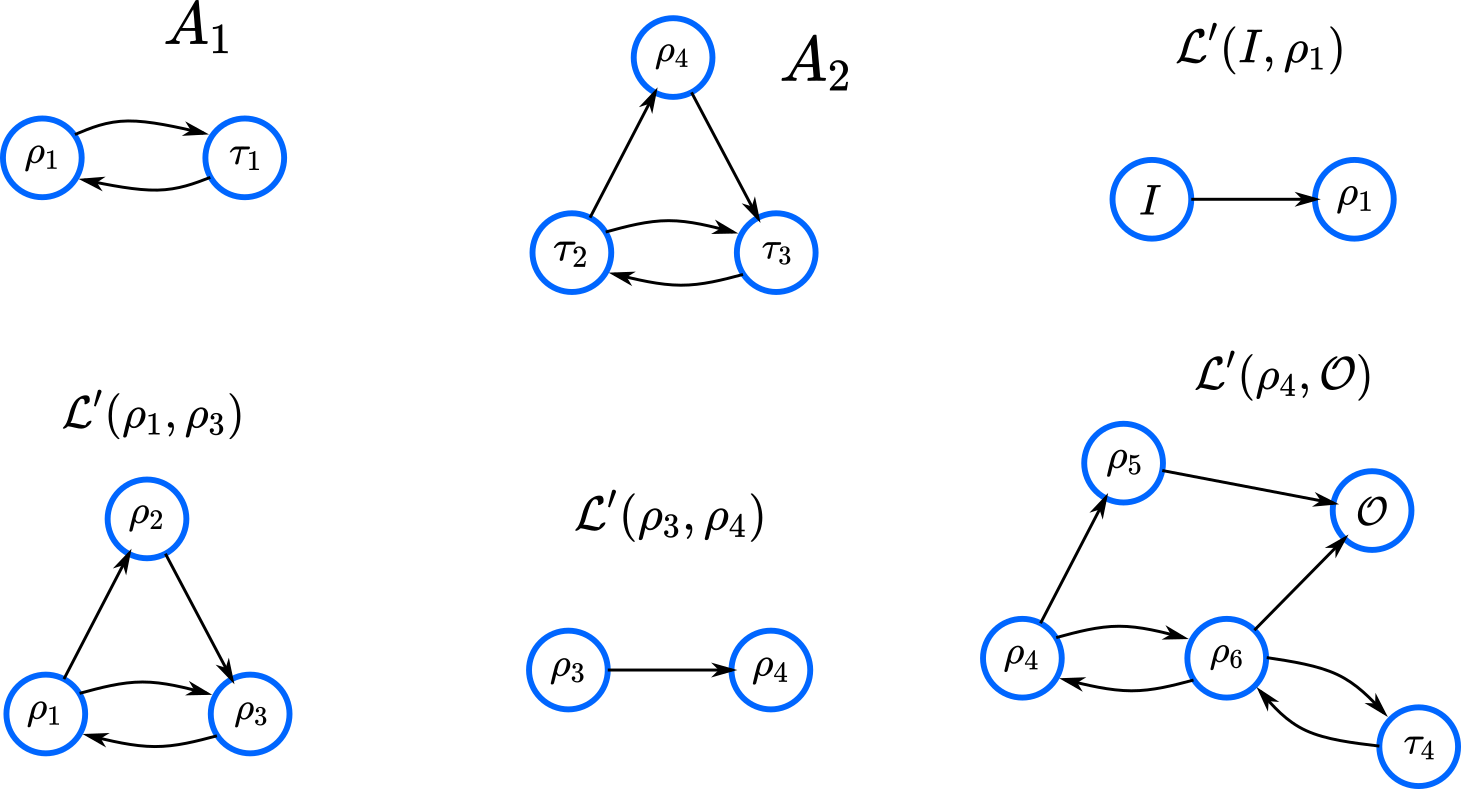
\includegraphics[scale=0.5]{figs/example_sec2_subnets.png}
    \caption{Homeostasis subnetworks of the 12-node network.}
    \label{fig:fig2}
\end{figure}